\documentclass{article}
% translate with >> pdflatex -shell-escape <file>

% This file is used as unit test for pgfplots, copyright by Christian Feuersaenger.
% 
% See
%   http://pgfplots.sourceforge.net/pgfplots.pdf
% for pgfplots.
%
% Any required input files (for <plot table> or <plot file> or the table package) can be downloaded
% at
% http://www.ctan.org/tex-archive/graphics/pgf/contrib/pgfplots/doc/latex/
% and
% http://www.ctan.org/tex-archive/graphics/pgf/contrib/pgfplots/doc/latex/plotdata/

\usepackage{pgfplots}
\pgfplotsset{compat=1.4}

\pagestyle{empty}

\begin{document}
\long\def\TESTS{%
	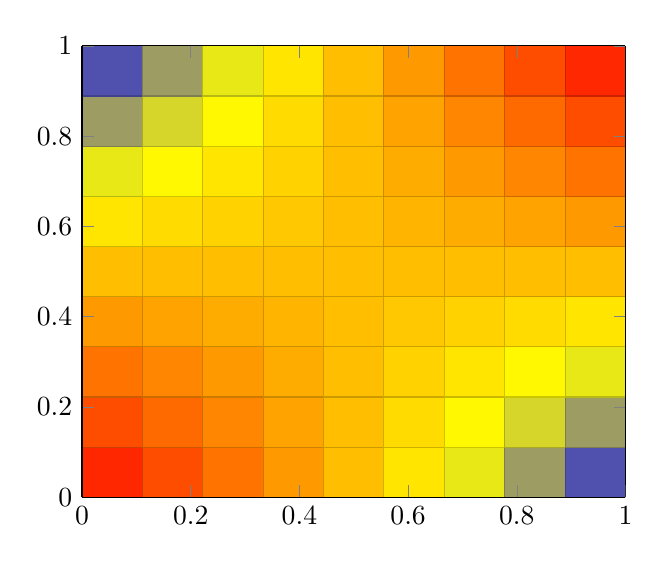
\begin{tikzpicture}
		\begin{axis}[view={0}{90}]
		\addplot3[surf,domain=0:1,samples=10] {(1-x)*(1-y) + x*y};
		\end{axis}
	\end{tikzpicture}

	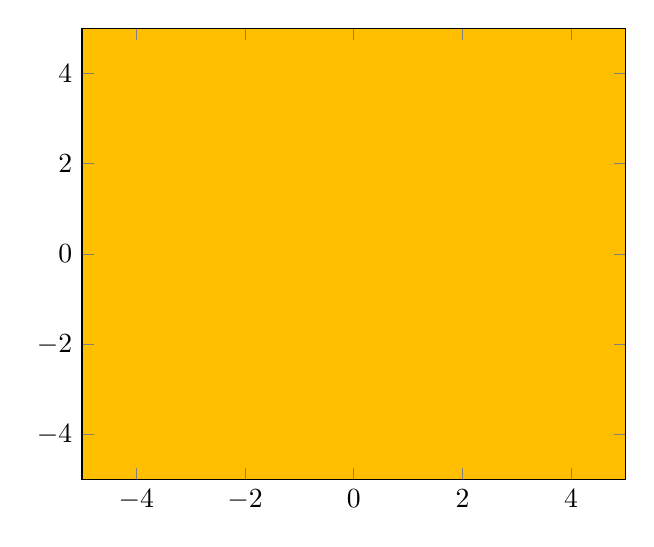
\begin{tikzpicture}
		\begin{axis}[view={0}{90}]
		\addplot3[surf,samples=2] {x*y};
		\end{axis}
	\end{tikzpicture}


	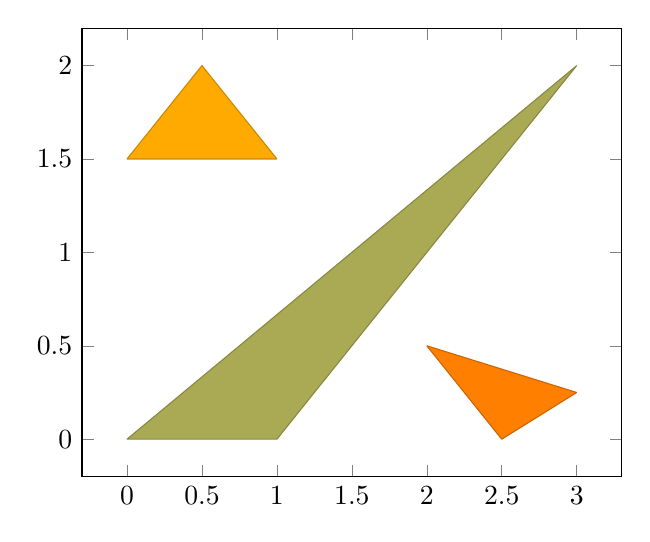
\begin{tikzpicture}
		\begin{axis}
			
		\addplot[patch,point meta=\thisrow{c}] table[row sep=\\] {
			x y c\\
			0 0 0\\
			1 0 0 \\
			3 2 2\\
			%\\
			0 1.5  1.5\\
			1 1.5  1.5\\
			0.5 2  2\\
			%\\
			2.5 0     1\\
			3 	0.25  2\\
			2 0.5     3\\
		}; 
		\end{axis}
	\end{tikzpicture}

	\begin{tikzpicture}
		\begin{axis}
		\addplot3[patch] file {plotdata/FokkerDrI_layer_0.patches.dat};
		\end{axis}
	\end{tikzpicture}



	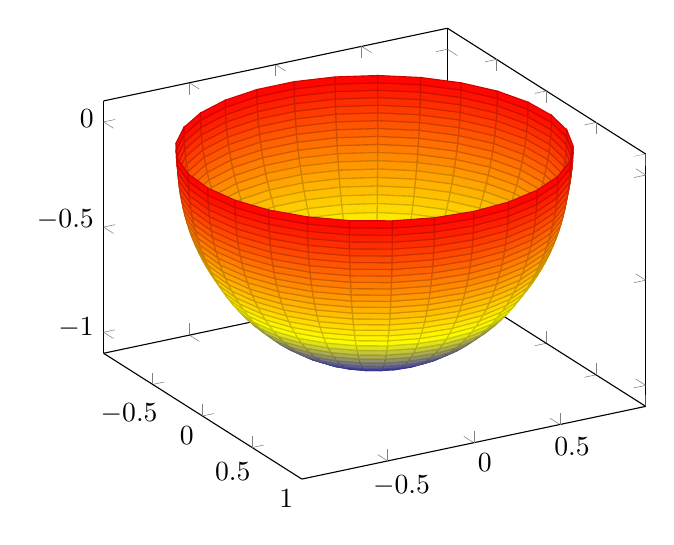
\begin{tikzpicture}
	\begin{axis}[view={60}{30}]
		\addplot3[surf,z buffer=sort,
			samples=30,domain=-1:0,y domain=0:2*pi]
			({sqrt(1-x^2) * cos(deg(y))},
			 {sqrt( 1-x^2 ) * sin(deg(y))},
			 x);
	\end{axis}
	\end{tikzpicture}

}

\subsection{shader=flat}
{
	\pgfplotsset{shader=flat}
	\TESTS
}

\subsection{shader=flat corner}
{
	\pgfplotsset{shader=flat corner}
	\TESTS
}

\subsection{shader=interp}
{
	\pgfplotsset{shader=interp}
	\TESTS
}

\subsection{shader=faceted interp}
{
	\pgfplotsset{shader=faceted interp}
	\TESTS
}
\end{document}
